
%\documentclass[paper]{geophysics}
\documentclass[manuscript,revised]{geophysics}
\usepackage{amsmath,amssymb}

% An example of defining macros
\newcommand{\rs}[1]{\mathstrut\mbox{\scriptsize\rm #1}}
\newcommand{\rr}[1]{\mbox{\rm #1}}

\begin{document}

\title{Estimating total magnetization direction using equivalent-layer technique}

\renewcommand{\thefootnote}{\fnsymbol{footnote}} 

\ms{GEO-2018XXXX} % manuscript number

\address{
\footnotemark[2] Observat\'orio Nacional, Rio de Janeiro, Brazil\\
\footnotemark[1] Corresponding author: reisandreluis@gmail.com}
\author{Andr\'e L. A. Reis\footnotemark[2] \footnotemark[1], Vanderlei C. Oliveira Jr.\footnotemark[2] and Val\'eria C. F. Barbosa \footnotemark[2]}

%\footer{Example}
\lefthead{Reis, A.L.A. \& Oliveira Jr, V.C. \& Barbosa, V. C. F.}
\righthead{Determining total magnetization direction}

\maketitle


\begin{abstract}
We developed a new method for estimating the total magnetization direction of magnetic sources based on equivalent-layer technique using total-field anomaly data. This approach does not impose strong information either about the shape or about the depth of the sources, and does not require a regularly spaced data. Usually, this equivalent-layer technique is used for processing total-field anomaly data by estimating a 2D magnetic-moment distribution over a fictitional layer composed by dipoles below the observation plane. When the magnetization direction of equivalent sources is almost the same as the true body, the estimated magnetic property over the layer is all positive. Iteratively, the proposed method imposes zeroth-order Tikhonov regularization and positivity constraint on the estimated magnetic moment over the layer and estimate the magnetization direction of the geological sources. Mathematically, the algorithm solves least-squares problems in two steps: the first one solves a linear inverse problem for estimating a 2D magnetic-moment distribution within the equivalent layer and the second solves a nonlinear inverse problem for magnetization direction of the magnetized sources. We test the methodology by applying to synthetic data for complicated geological scenarios, and the results show that the method can be a powerful tool for estimating the magnetization direction of a set of bodies. Tests on field data from Goias Alkaline Province (GAP), center of Brazil, over Montes Claros complex suggests intrusions with remarkable strong remanent magnetization, in agreement with the current literature for this region. 
\end{abstract}
%\section{Introduction}

%% Brief introduction
One of the earliest geophysical method used in petroleum and mining exploration is the magnetic method. This method has been applied for interpreting a wide range of geological scenarios like estimating the basement relief, mapping faults and lithological contacts, defining bounds and shapes of geological sources and determining the position of salt domes whithin sediments. However, to retrieve the shape of magnetized geological sources with reasonable confidence from total-field anomaly, it is necessary to use a reliable information about the magnetization direction. 

%% The importance of magnetization direction and techniques
Most of  magnetic methods require knowledge of the magnetization direction, otherwise they yield unsatisfactory interpretations of the exploration targets. This fact has been propelled the development of several techniques for estimating magnetization direction over the last 50 years. The strategies for estimating this quantity can be divided into two main groups. The first one comprises the methods which presume a prior information about the shape of geological sources. \cite{bhattacharyya1966} presented an iterative method for determining the parameters of a rectangular prismatic shape, such as horizontal dimensions, depth of the body and magnetization direction. \cite{emilia_massey_1974} approximate the a seamount by a set of stacked prisms with the same magnetization direction and different magnetization intensity. \cite{parker_etal_1987} proposed a method for estimating de magnetization direction formulating as an optimization problem by imposing an uniformly magnetization distribution. \cite{kubota2005} also parametrized a seamoumt approximating by a set of juxtaposed prisms and estimating the magnetization direction of each one. Finally, \cite{oliveirajr_etal_2015} approximate a magnetic source by a spherical geometry, assumig the knowledge of the center and estimating the magnetization direction. The second group are the methods which not presume any information about the magnetic source. \cite{fedi_etal_1994}, for example, proposed a method that performs a succesive reduction-to-pole on frequency domain testing it for a set of magnetization direction. \cite{medeiros_silva_1995} presented an interpretation method that estimates the total magnetization direction and the spatial orientation of the source based on the multipole expansion. \cite{phillips2005} implemented an algorithm that uses the Helbig's integral for estimating the three-component vector of the magnetic-dipole moment. \cite{tontini_pedersen_2008} extended the method using the same Helbig's integral to estimate the magnetization direction and its magnitude, also providing information about the position of the center of magnetization distribution. \cite{lelievre_oldenburg_2009} developed a method for estimating the magnetization direction in complex geological scenarios. In addition, there are the methods that are based on the correlation of potential quantities \citep[e.g.,][]{dannemiller_li_2006,gerovska_etal_2009,liu_etal_2015,zhang_etal_2018}.

%%The equivalent layer 
Estimating the magnetization direction is extremely important not only for interpretation, but also for processing the total-field anomaly data. One technique in spatial domain commonly used for processing potential-field data is the equivalent layer. It was first introduced by \cite{dampney1969} and \cite{emilia_massey_1974} for processing gravity and magnetic data, respectively. After these pioneer works, this technique has been widely used for processing such as interpolation \citep{cordell_1992,mendonca-silva_1994,barnes-lumley_2011,siqueira_etal_2017}, upward (or downward) continuation  \citep{hansen-miyazaki_1984,li-oldenburg_2010}, reduction to the pole \citep{silva_1986,leao-silva_1989,guspi-novara_2009,oliveirajr-etal_2013}, computing the amplitude of anomalous field \citep{li_li_2014} and denoising gradient data \citep{martinez_li_2016}. The equivalent layer approach consists in approximating the observed and predicted data produced by a set of discrete sources (e.g., prisms, dipoles or point masses) commonly known as equivalent sources. Once the physical-property distribution within an equivalent layer is estimated, it has been usually used for processing and it has been much less used in interpreting potential-field data. 

%%  positivity constraints 
In scanning magnetic microscopy the equivalent-layer technique is usually used in interpreting the magnetic material over thin sections of rock samples because the shape of the true source (a thin-section of rock) resembles the layer of equivalent sources. \cite{weiss2007}, using magnetic microscopy data, pointed out that fixing a magnetization direction the estimated magnetic moment on the layer are all-positive if the magnetization direction is equal to the one used to magnetized the rock sample artificially. \cite{baratchart2013} show that, assuming the unidirectional solution, its possible to achieve uniqueness on the inverse problem. \cite{lima2013} proposed a method on the frequency domain to investigate the unidirectional solution on a thin-section of geological sample with magnetic microscopy data, showing that the estimated physical-property over the layer is entirely positive. On the other hand, in the geophysical exploration works, the equivalent-layer technique is usually used for processing potential-field data. Under this perspective, there is no relationship between the physical-property distribution on the equivalent layer and the true geologic sources. Hence, the layer is just a mathematical abstraction devoid of a geologically meaningful result. A few authors in geophysical exploration literature have been addressed the use of the equivalent-layer technique in the interpretation of the geologic sources. \cite{pedersen1991}, for example, discussed the relation between potential field and equivalent source. \cite{medeiros_silva1996} and \cite{silvadias_etal_2010} estimated an apparent-magnetization map on a layer by using Tikhonov and entropic regularizations respectively. \cite{siqueira_etal_2017} established a relationship between the excess of mass estimated over the equivalent layer and the true one. \cite{li_nabighian_oldenburg_2014} using total-field anomaly data, proved the existence of a positive distribution over the layer, and its a sufficient feature to overcome the low-latitude instability. However, these authors considered only a purely induced magnetization for the magnetic sources.

%% Joining techniques for estimating the magnetization direction 
Here, we mathematically prove that the all-positive magnetic-moment distribution within an equivalent layer exists even in the presence of remanent magnetization of the true geologic sources. This all-positive magnetic-moment distribution holds true for all cases in which the magnetization direction of the equivalent sources over the layer has the same direction as the magnetization direction of the true geologic sources, regardless of whether the magnetization of the true sources is purely induced or not. Grounded on this theoretical aspect, we present a new method using total-field anomaly data that estimates the magnetization direction without presume any information about the magnetic sources. Our method consists of two nested algorithm to solve the inverse problem estimating the magnetic-moment distribution within an equivalent layer subjected to a positivity constraint and a regularized function and the magnetization direction. We examine the performance of the method testing it in synthetic tests generated by different geological scenarios. Furthermore, application to field data from Goi\'as alkaline province (GAP) over the Montes Claros complex, center of Brazil, shows the performance of the method in estimating a meaningful magnetization direction. The result suggests the presence of a remarkable remanent magnetization.    



\section{Methodology}
\label{sec:methodology}

% % Explaining the continuous magnetic equivalent layer  

Considering a Cartesian coordinate system with $x$-, $y$- and $z$-axis being oriented to north, east and downward, respectively. Let $\Delta T_i \equiv \Delta T (x_i,y_i,z_i)$ be the total field anomaly, at the $i$-th position $(x_i,y_i,z_i)$, produced by a continuos layer located below the observation plane on the depth $z_c$, where $z_c > z_i$, and $p(x',y',z_c)$ is the distribution of magnetic dipoles per unit area over the layer surface. In this case, the total field anomaly produced by this continuous layer is given by the equation 

\begin{equation}
\Delta T_i = \int \limits_{-\infty}^{+\infty } \int \limits_{-\infty}^{+\infty }  p(x',y',z_c)  [\gamma_m \hat{\mathbf{F}}_0^T \mathbf{H} \,\hat{\mathbf{h}}(\mathbf{q})] dx' \,dy',
\label{eq:continuous_layer}
\end{equation}
where $\gamma_m$ is a constant proportional to the vaccum permeability, $\hat{\mathbf{F}}_0$ is a unit vector with the same direction of the geomagnetic field $\mathbf{F}_0$ and $\mathbf{H}$ is a $3 \times 3$ matrix equal to  

 \begin{equation}
   \mathbf{H} =
   \left[ \begin{array}{ccc}
   \partial_{xx} \phi & \partial_{xy} \phi &\partial_{xz} \phi \\  \partial_{yx} \phi & \partial_{yy} \phi &\partial_{yz} \phi \\  \partial_{zx} \phi &\partial_{zy}\phi  & \partial_{zz} \phi    
   \end{array} \right] ,
   \label{eq:H}
 \end{equation}
where $\partial_{\alpha \beta}\phi$, $\alpha = x, y, z$, $\beta = x, y, z$, is the second derivative of the function 

\begin{equation}
   \phi (x-x', y-y', z-z_c) = \frac{1}{r} ,
   \label{eq:phi}
 \end{equation}
where $r = [(x-x')^2 + (y-y')^2 + (z-z_c)^2]^{1/2}$ and $\hat{\mathbf{h}}(\mathbf{q})$ is a unit vector with the
magnetization direction of the layer that depends on the vector $\mathbf{q}$ given by 

 \begin{equation}
   \mathbf{q} =
   \left[ \begin{array}{c}
   i  \\ 
   d     
   \end{array} \right] ,
   \label{eq:q_vector}
 \end{equation}
 where $i$ and $d$ is the inclination and declination, respectively.

% % Formulating foward problem 


According the equivalent layer technique theory, we can produce the a set of $N$ total field anomaly 
observations generated by a 3D magnetic source by a layer. 


By discretizing 

%It is worth pointing out that the equivalent source is represented by a dipole with unit volume

%$\mathbf{p}$ is the \textit{M}-dimensional vector defined as parameter vector whose $j$th element is the magnetic intensity of the $j$th equivalent source

%$\mathbf{q}$ is a $2 \times 1 $ vector containing the inclination and the declination of the equivalent dipoles 
  

%We consider that the $M$ equivalent sources are distributed with a constant depth $h$ below the observation plane, forming an equivalent layer 

%Mathematically, the effect produced by the equivalent layer at $N$ observation points can be given as  

% % Formulating the inverse problem explaining the iterative method

%Let $\mathbf{\Delta T}^o$ be an \textit{N}-dimensional vector whose $i$th element is the total field anomaly observation produced by a magnetic source at the point $(x_i,y_i,z_i)$, $i = 1, \ldots, N$. 

% % Constraining the magnetic moment of equivalent sources

% % Practical Procedures 

% % Generalization of all-positive equivalent sources 






\newpage

\bibliographystyle{seg}  % style file is seg.bst
\bibliography{example}

\clearpage

%% Generatinf for the methodology

\begin{figure}
	\centering
	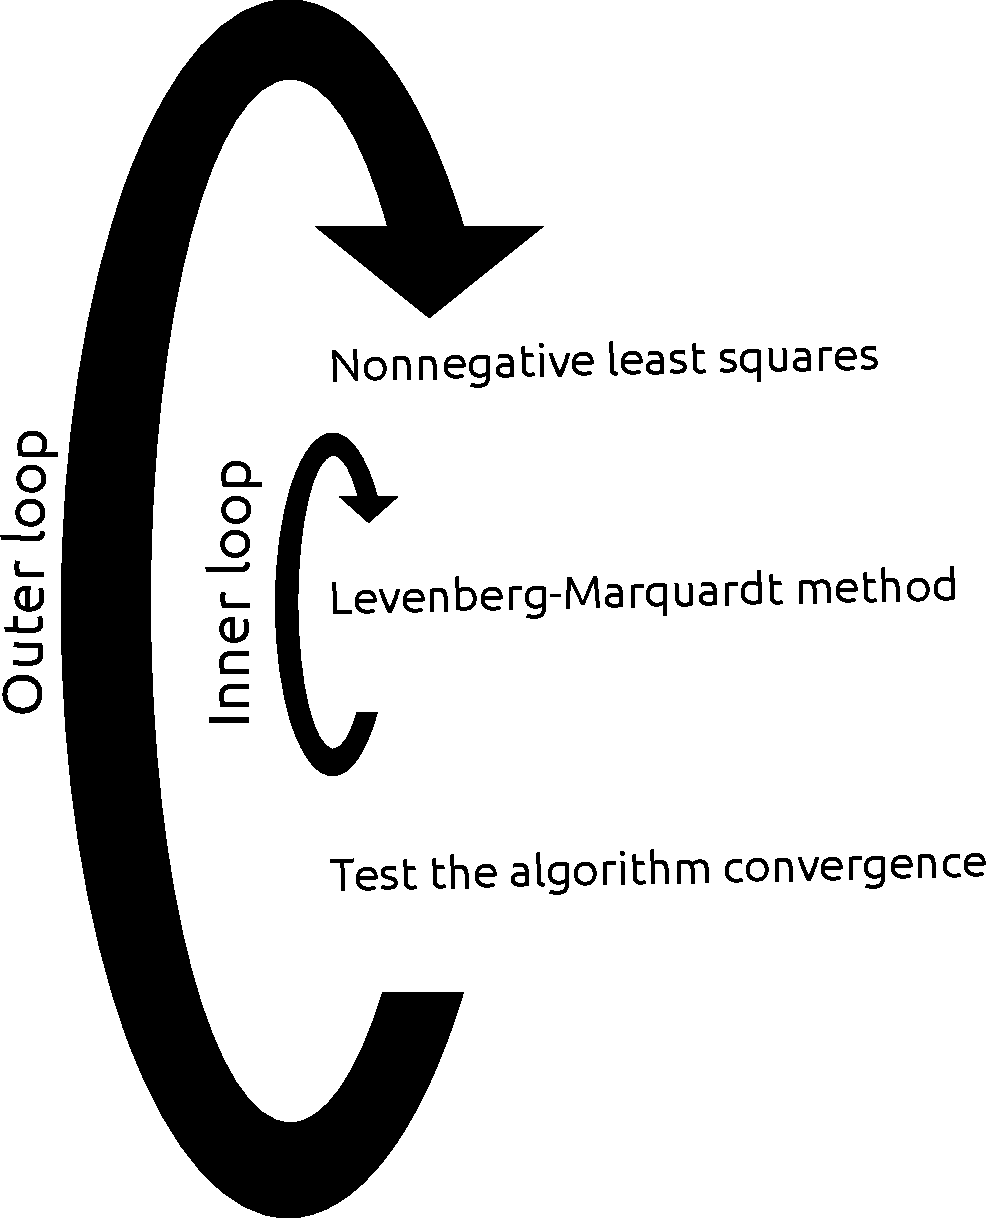
\includegraphics[width=0.6\textwidth]{Fig/algorithm_LM_NNLS.pdf}
	\caption{Iterative scheme overview for NNLS and Levenberg-Marquardt method for estimating magnetization direction. The outer loop is the nonnegative solution for magnetic-moment distribution and the inner loop calculates the magnetization direction using Levenberg-Marquardt method.}
	\label{fig:scheme_LM_NNLS}
\end{figure}


\end{document}
